\documentclass{standalone}
\usepackage{tikz}
\usetikzlibrary{patterns, positioning}

\begin{document}
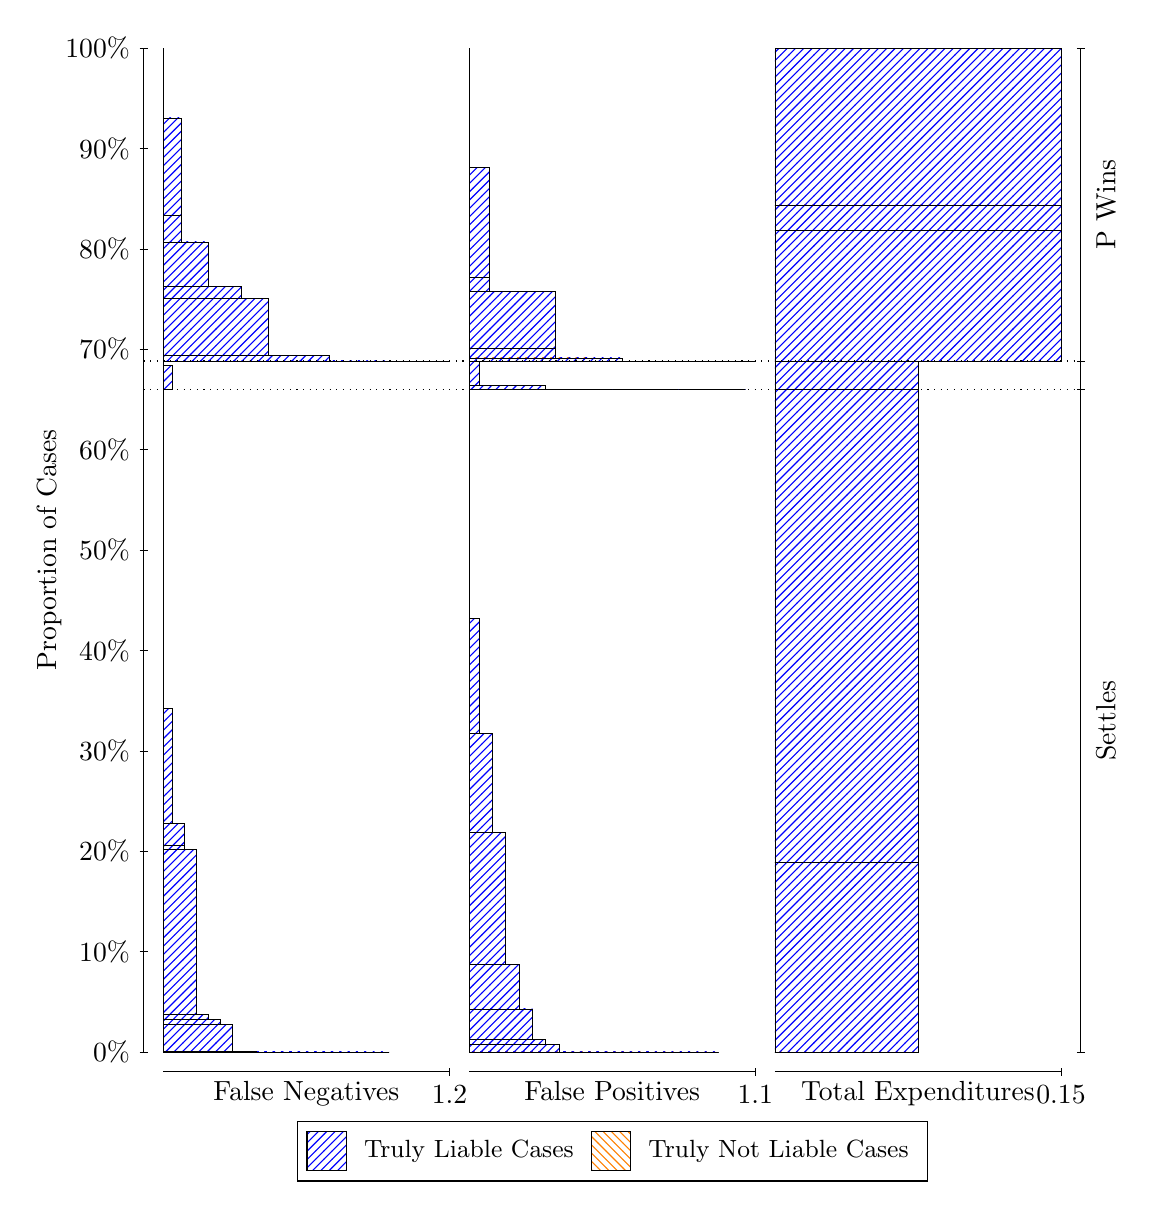
\begin{tikzpicture}
\draw[black, very thin] (1.5,1.75) -- (1.5,14.5);
\node[rotate=90, anchor=center] at (0.3, 8.125) {Proportion of Cases};
\draw[black, very thin] (1.45,1.75) -- (1.55,1.75);
\node[anchor=east] at (1.45, 1.75) {0\%};
\draw[black, very thin] (1.45,3.025) -- (1.55,3.025);
\node[anchor=east] at (1.45, 3.025) {10\%};
\draw[black, very thin] (1.45,4.3) -- (1.55,4.3);
\node[anchor=east] at (1.45, 4.3) {20\%};
\draw[black, very thin] (1.45,5.575) -- (1.55,5.575);
\node[anchor=east] at (1.45, 5.575) {30\%};
\draw[black, very thin] (1.45,6.85) -- (1.55,6.85);
\node[anchor=east] at (1.45, 6.85) {40\%};
\draw[black, very thin] (1.45,8.125) -- (1.55,8.125);
\node[anchor=east] at (1.45, 8.125) {50\%};
\draw[black, very thin] (1.45,9.4) -- (1.55,9.4);
\node[anchor=east] at (1.45, 9.4) {60\%};
\draw[black, very thin] (1.45,10.675) -- (1.55,10.675);
\node[anchor=east] at (1.45, 10.675) {70\%};
\draw[black, very thin] (1.45,11.95) -- (1.55,11.95);
\node[anchor=east] at (1.45, 11.95) {80\%};
\draw[black, very thin] (1.45,13.225) -- (1.55,13.225);
\node[anchor=east] at (1.45, 13.225) {90\%};
\draw[black, very thin] (1.45,14.5) -- (1.55,14.5);
\node[anchor=east] at (1.45, 14.5) {100\%};

\draw[black, very thin] (13.4,1.75) -- (13.4,14.5);
\draw[black, very thin] (13.35,1.75) -- (13.45,1.75);
\node[anchor=west] at (13.35, 1.75) {};
\draw[black, very thin] (13.35,10.161) -- (13.45,10.161);
\node[anchor=west] at (13.35, 10.161) {};
\draw[black, very thin] (13.35,10.525) -- (13.45,10.525);
\node[anchor=west] at (13.35, 10.525) {};
\draw[black, very thin] (13.35,14.5) -- (13.45,14.5);
\node[anchor=west] at (13.35, 14.5) {};

\draw[black, very thin, pattern color=blue, pattern=north east lines] (1.75,1.75) rectangle (4.6184,1.75);
\draw[black, very thin, pattern color=blue, pattern=north east lines] (1.75,1.75) rectangle (4.3125,1.75);
\draw[black, very thin, pattern color=blue, pattern=north east lines] (1.75,1.75) rectangle (4.0065,1.75);
\draw[black, very thin, pattern color=blue, pattern=north east lines] (1.75,1.75) rectangle (3.8535,1.75);
\draw[black, very thin, pattern color=blue, pattern=north east lines] (1.75,1.75) rectangle (3.7005,1.75);
\draw[black, very thin, pattern color=blue, pattern=north east lines] (1.75,1.75) rectangle (3.5475,1.75);
\draw[black, very thin, pattern color=blue, pattern=north east lines] (1.75,1.75) rectangle (3.3946,1.7509);
\draw[black, very thin, pattern color=blue, pattern=north east lines] (1.75,1.7509) rectangle (3.2416,1.7509);
\draw[black, very thin, pattern color=blue, pattern=north east lines] (1.75,1.7509) rectangle (3.0886,1.7511);
\draw[black, very thin, pattern color=blue, pattern=north east lines] (1.75,1.7511) rectangle (2.9356,1.7511);
\draw[black, very thin, pattern color=blue, pattern=north east lines] (1.75,1.7511) rectangle (2.9356,1.754);
\draw[black, very thin, pattern color=blue, pattern=north east lines] (1.75,1.754) rectangle (2.7826,1.7573);
\draw[black, very thin, pattern color=blue, pattern=north east lines] (1.75,1.7573) rectangle (2.6296,2.0976);
\draw[black, very thin, pattern color=blue, pattern=north east lines] (1.75,2.0976) rectangle (2.4767,2.1636);
\draw[black, very thin, pattern color=blue, pattern=north east lines] (1.75,2.1636) rectangle (2.3237,2.2298);
\draw[black, very thin, pattern color=blue, pattern=north east lines] (1.75,2.2298) rectangle (2.1707,2.2298);
\draw[black, very thin, pattern color=blue, pattern=north east lines] (1.75,2.2298) rectangle (2.1707,4.3245);
\draw[black, very thin, pattern color=blue, pattern=north east lines] (1.75,4.3245) rectangle (2.0177,4.3783);
\draw[black, very thin, pattern color=blue, pattern=north east lines] (1.75,4.3783) rectangle (2.0177,4.6529);
\draw[black, very thin, pattern color=blue, pattern=north east lines] (1.75,4.6529) rectangle (1.8647,6.1154);
\draw[black, very thin, pattern color=orange, pattern=north west lines] (1.75,6.1154) rectangle (1.75,6.1154);
\draw[black, very thin, pattern color=blue, pattern=north east lines] (1.75,6.1154) rectangle (1.75,10.161);
\draw[black, very thin, pattern color=blue, pattern=north east lines] (1.75,10.161) rectangle (1.8647,10.47);
\draw[black, very thin, pattern color=orange, pattern=north west lines] (1.75,10.47) rectangle (1.75,10.47);
\draw[black, very thin, pattern color=blue, pattern=north east lines] (1.75,10.47) rectangle (1.75,10.525);
\draw[black, very thin, pattern color=blue, pattern=north east lines] (1.75,10.525) rectangle (5.3833,10.525);
\draw[black, very thin, pattern color=blue, pattern=north east lines] (1.75,10.525) rectangle (4.6184,10.526);
\draw[black, very thin, pattern color=blue, pattern=north east lines] (1.75,10.526) rectangle (4.2742,10.526);
\draw[black, very thin, pattern color=blue, pattern=north east lines] (1.75,10.526) rectangle (3.8535,10.597);
\draw[black, very thin, pattern color=blue, pattern=north east lines] (1.75,10.597) rectangle (3.5093,10.597);
\draw[black, very thin, pattern color=blue, pattern=north east lines] (1.75,10.597) rectangle (3.0886,11.321);
\draw[black, very thin, pattern color=blue, pattern=north east lines] (1.75,11.321) rectangle (2.7444,11.323);
\draw[black, very thin, pattern color=blue, pattern=north east lines] (1.75,11.323) rectangle (2.7444,11.47);
\draw[black, very thin, pattern color=blue, pattern=north east lines] (1.75,11.47) rectangle (2.3237,12.038);
\draw[black, very thin, pattern color=blue, pattern=north east lines] (1.75,12.038) rectangle (1.9795,12.379);
\draw[black, very thin, pattern color=blue, pattern=north east lines] (1.75,12.379) rectangle (1.9795,13.612);
\draw[black, very thin, pattern color=orange, pattern=north west lines] (1.75,13.612) rectangle (1.75,13.612);
\draw[black, very thin, pattern color=blue, pattern=north east lines] (1.75,13.612) rectangle (1.75,14.5);
\draw[black, very thin, pattern color=orange, pattern=north west lines] (5.6333,1.75) rectangle (8.8019,1.75);
\draw[black, very thin, pattern color=blue, pattern=north east lines] (5.6333,1.75) rectangle (8.8019,1.75);
\draw[black, very thin, pattern color=orange, pattern=north west lines] (5.6333,1.75) rectangle (8.126,1.75);
\draw[black, very thin, pattern color=blue, pattern=north east lines] (5.6333,1.75) rectangle (8.126,1.75);
\draw[black, very thin, pattern color=blue, pattern=north east lines] (5.6333,1.75) rectangle (7.957,1.75);
\draw[black, very thin, pattern color=orange, pattern=north west lines] (5.6333,1.75) rectangle (7.788,1.75);
\draw[black, very thin, pattern color=blue, pattern=north east lines] (5.6333,1.75) rectangle (7.788,1.75);
\draw[black, very thin, pattern color=orange, pattern=north west lines] (5.6333,1.75) rectangle (7.45,1.75);
\draw[black, very thin, pattern color=blue, pattern=north east lines] (5.6333,1.75) rectangle (7.45,1.75);
\draw[black, very thin, pattern color=blue, pattern=north east lines] (5.6333,1.75) rectangle (7.281,1.75);
\draw[black, very thin, pattern color=orange, pattern=north west lines] (5.6333,1.75) rectangle (7.112,1.75);
\draw[black, very thin, pattern color=blue, pattern=north east lines] (5.6333,1.75) rectangle (7.112,1.7512);
\draw[black, very thin, pattern color=orange, pattern=north west lines] (5.6333,1.7512) rectangle (7.112,1.7512);
\draw[black, very thin, pattern color=blue, pattern=north east lines] (5.6333,1.7512) rectangle (7.112,1.7512);
\draw[black, very thin, pattern color=blue, pattern=north east lines] (5.6333,1.7512) rectangle (6.943,1.7512);
\draw[black, very thin, pattern color=orange, pattern=north west lines] (5.6333,1.7512) rectangle (6.774,1.7512);
\draw[black, very thin, pattern color=blue, pattern=north east lines] (5.6333,1.7512) rectangle (6.774,1.8437);
\draw[black, very thin, pattern color=blue, pattern=north east lines] (5.6333,1.8437) rectangle (6.605,1.9075);
\draw[black, very thin, pattern color=orange, pattern=north west lines] (5.6333,1.9075) rectangle (6.436,1.9075);
\draw[black, very thin, pattern color=blue, pattern=north east lines] (5.6333,1.9075) rectangle (6.436,2.2944);
\draw[black, very thin, pattern color=blue, pattern=north east lines] (5.6333,2.2944) rectangle (6.436,2.2964);
\draw[black, very thin, pattern color=blue, pattern=north east lines] (5.6333,2.2964) rectangle (6.2671,2.8608);
\draw[black, very thin, pattern color=blue, pattern=north east lines] (5.6333,2.8608) rectangle (6.2671,2.8608);
\draw[black, very thin, pattern color=orange, pattern=north west lines] (5.6333,2.8608) rectangle (6.0981,2.8608);
\draw[black, very thin, pattern color=blue, pattern=north east lines] (5.6333,2.8608) rectangle (6.0981,4.5397);
\draw[black, very thin, pattern color=blue, pattern=north east lines] (5.6333,4.5397) rectangle (6.0981,4.5403);
\draw[black, very thin, pattern color=blue, pattern=north east lines] (5.6333,4.5403) rectangle (5.9291,5.7958);
\draw[black, very thin, pattern color=blue, pattern=north east lines] (5.6333,5.7958) rectangle (5.7601,7.2583);
\draw[black, very thin, pattern color=blue, pattern=north east lines] (5.6333,7.2583) rectangle (5.6333,10.161);
\draw[black, very thin, pattern color=orange, pattern=north west lines] (5.6333,10.161) rectangle (9.1399,10.161);
\draw[black, very thin, pattern color=blue, pattern=north east lines] (5.6333,10.161) rectangle (9.1399,10.161);
\draw[black, very thin, pattern color=blue, pattern=north east lines] (5.6333,10.161) rectangle (8.295,10.161);
\draw[black, very thin, pattern color=blue, pattern=north east lines] (5.6333,10.161) rectangle (7.45,10.161);
\draw[black, very thin, pattern color=blue, pattern=north east lines] (5.6333,10.161) rectangle (6.605,10.216);
\draw[black, very thin, pattern color=blue, pattern=north east lines] (5.6333,10.216) rectangle (5.7601,10.525);
\draw[black, very thin, pattern color=orange, pattern=north west lines] (5.6333,10.525) rectangle (9.2667,10.525);
\draw[black, very thin, pattern color=blue, pattern=north east lines] (5.6333,10.525) rectangle (9.2667,10.525);
\draw[black, very thin, pattern color=orange, pattern=north west lines] (5.6333,10.525) rectangle (8.4217,10.525);
\draw[black, very thin, pattern color=blue, pattern=north east lines] (5.6333,10.525) rectangle (8.4217,10.525);
\draw[black, very thin, pattern color=orange, pattern=north west lines] (5.6333,10.525) rectangle (7.5767,10.525);
\draw[black, very thin, pattern color=blue, pattern=north east lines] (5.6333,10.525) rectangle (7.5767,10.566);
\draw[black, very thin, pattern color=orange, pattern=north west lines] (5.6333,10.566) rectangle (7.1965,10.566);
\draw[black, very thin, pattern color=blue, pattern=north east lines] (5.6333,10.566) rectangle (7.1965,10.566);
\draw[black, very thin, pattern color=orange, pattern=north west lines] (5.6333,10.566) rectangle (6.7318,10.566);
\draw[black, very thin, pattern color=blue, pattern=north east lines] (5.6333,10.566) rectangle (6.7318,10.686);
\draw[black, very thin, pattern color=blue, pattern=north east lines] (5.6333,10.686) rectangle (6.7318,11.412);
\draw[black, very thin, pattern color=orange, pattern=north west lines] (5.6333,11.412) rectangle (6.3516,11.412);
\draw[black, very thin, pattern color=blue, pattern=north east lines] (5.6333,11.412) rectangle (6.3516,11.413);
\draw[black, very thin, pattern color=blue, pattern=north east lines] (5.6333,11.413) rectangle (5.8868,11.584);
\draw[black, very thin, pattern color=blue, pattern=north east lines] (5.6333,11.584) rectangle (5.8868,12.986);
\draw[black, very thin, pattern color=orange, pattern=north west lines] (5.6333,12.986) rectangle (5.6333,12.986);
\draw[black, very thin, pattern color=blue, pattern=north east lines] (5.6333,12.986) rectangle (5.6333,14.5);
\draw[black, very thin, pattern color=orange, pattern=north west lines] (9.5167,1.75) rectangle (11.333,1.75);
\draw[black, very thin, pattern color=blue, pattern=north east lines] (9.5167,1.75) rectangle (11.333,4.1542);
\draw[black, very thin, pattern color=orange, pattern=north west lines] (9.5167,4.1542) rectangle (11.333,4.1542);
\draw[black, very thin, pattern color=blue, pattern=north east lines] (9.5167,4.1542) rectangle (11.333,10.161);
\draw[black, very thin, pattern color=orange, pattern=north west lines] (9.5167,10.161) rectangle (11.333,10.161);
\draw[black, very thin, pattern color=blue, pattern=north east lines] (9.5167,10.161) rectangle (11.333,10.525);
\draw[black, very thin, pattern color=orange, pattern=north west lines] (9.5167,10.525) rectangle (13.15,10.525);
\draw[black, very thin, pattern color=blue, pattern=north east lines] (9.5167,10.525) rectangle (13.15,12.182);
\draw[black, very thin, pattern color=orange, pattern=north west lines] (9.5167,12.182) rectangle (13.15,12.182);
\draw[black, very thin, pattern color=blue, pattern=north east lines] (9.5167,12.182) rectangle (13.15,12.508);
\draw[black, very thin, pattern color=orange, pattern=north west lines] (9.5167,12.508) rectangle (13.15,12.508);
\draw[black, very thin, pattern color=blue, pattern=north east lines] (9.5167,12.508) rectangle (13.15,14.5);
\draw[black, dotted] (1.5,10.161) -- (13.4,10.161);
\draw[black, dotted] (1.5,10.525) -- (13.4,10.525);
\draw[black, very thin] (1.75,1.5) -- (5.3833,1.5);
\node[anchor=north] at (3.5667, 1.5) {False Negatives};
\draw[black, very thin] (5.3833,1.45) -- (5.3833,1.55);
\node[anchor=north] at (5.3833, 1.45) {1.2};

\draw[black, very thin] (5.6333,1.5) -- (9.2667,1.5);
\node[anchor=north] at (7.45, 1.5) {False Positives};
\draw[black, very thin] (9.2667,1.45) -- (9.2667,1.55);
\node[anchor=north] at (9.2667, 1.45) {1.1};

\draw[black, very thin] (9.5167,1.5) -- (13.15,1.5);
\node[anchor=north] at (11.333, 1.5) {Total Expenditures};
\draw[black, very thin] (13.15,1.45) -- (13.15,1.55);
\node[anchor=north] at (13.15, 1.45) {0.15};

\node[black, centered, rotate=90] at (13.72, 5.9556) {Settles};

\node[black, centered, rotate=90] at (13.72, 12.512) {P Wins};

\draw (7.449999999999999,1.5) node[draw=none] (baseCoordinate) {};
\begin{scope}[align=center]
        \matrix[scale=0.5, draw=black, below=0.5cm of baseCoordinate, nodes={draw}, column sep=0.1cm]{
            \node[rectangle, draw, minimum width=0.5cm, minimum height=0.5cm, pattern=north east lines, pattern color=blue] {}; &
            \node[draw=none, font=\small] (B) {Truly Liable Cases}; &
            \node[rectangle, draw, minimum width=0.5cm, minimum height=0.5cm, pattern=north west lines, pattern color=orange] {}; &
            \node[draw=none, font=\small] (B) {Truly Not Liable Cases}; \\
            };
\end{scope}

\end{tikzpicture}
\end{document}